\documentclass[11pt]{article}
\usepackage[margin=1in]{geometry}
\usepackage{amsmath,amssymb,graphicx,listings,xcolor,float}
\usepackage{enumitem}
\usepackage{epstopdf}

\lstset{
  language=Matlab,
  basicstyle=\small\ttfamily,
  keywordstyle=\color{blue},
  commentstyle=\color{green!50!black},
  stringstyle=\color{red},
  numbers=left,
  numberstyle=\tiny\color{gray},
  breaklines=true,
  frame=single,
  tabsize=4
}

\title{MATH 543 -- Homework 6}
\author{Parham Khodadi}
\date{}

\begin{document}
\maketitle

%% ============================================================
\section*{TB-18.1}
%% ============================================================

\subsection*{Problem}
Consider the example $A = \begin{bmatrix} 1 & 1 \\ 1 & 1.0001 \\ 1 & 1.0001 \end{bmatrix}$, $\vec{b} = \begin{bmatrix} 2 \\ 0.0001 \\ 4.0001 \end{bmatrix}$.

\begin{enumerate}[label=\Alph*)]
    \item What are the matrices $A^+$ and $P$ for this example? Give exact answers.
    \item Find the exact solutions $x$ and $y=Ax$ to the least squares problem $Ax \approx b$.
    \item What are $\kappa(A)$, $\theta$, and $\eta$? From here on, numerical answers are acceptable.
    \item What are the four conidition numbers of Theorem 18.1?
    \item Give examples of perturbations $\delta b$ and $\delta A$ that approximately attain these four condition numbers.
\end{enumerate}

\subsection*{Solution}
MATLAB code found in Appendix.

\subsubsection*{A)}
$A^+ = (A^T A)^{-1} A^T = \begin{bmatrix}
    10001 & -5000 & -5000 \\
    -10000 & 5000 & 5000 
\end{bmatrix}$

$P = AA^+ = \begin{bmatrix}
    1 & 0 & 0 \\
    0 & 0.5 & 0.5 \\
    0 & 0.5 & 0.5    
\end{bmatrix}$

\subsubsection*{B)}
$\vec{x} = A^+ \vec{b}=\begin{bmatrix}
    1 \\ 1
\end{bmatrix}$

$\vec{y} = A \vec{x} = \begin{bmatrix}
    2 \\ 2.0001 \\ 2.0001
\end{bmatrix}$

\newpage
\subsubsection*{C)}
$\kappa(A) = \frac{\sigma_1}{\sigma_n} \approx 42429.235416083058$

$\theta = cos^{-1}(\frac{||\vec{y}||_2}{||\vec{b}||_2}) \approx 0.68470283674839516 rad \approx 39.2305827663180509\deg$

$\eta = \frac{||A||_2 ||\vec{x}||_2}{||\vec{y}||_2} \approx 1.0000000005535632$

\subsubsection*{D)}
$\kappa(b \rightarrow{} y) = 1.2909771975928801$

$\kappa(b \rightarrow{} x) = 54775.175403141970$

$\kappa(A \rightarrow{} y) = 54775.175433463490$

$\kappa(A \rightarrow{} x) = 1469883143.3101680$

\subsubsection*{E)}
I wasn't sure how to do this part, so I asked Gemini for help. Check the Appendix for more info.

To approximately attain these four condition numbers, we construct specific worst-case perturbations using the Singular Value Decomposition $A = U \Sigma V^T$ and the residual $\vec{r} = \vec{b} - \vec{y}$. Let $\epsilon > 0$ be a small scaling scalar (e.g., $10^{-8}$). 

\begin{itemize}
    \item \textbf{$\kappa(b \rightarrow y)$:} The perturbation $\delta b$ must lie entirely in the column space of $A$. We choose $\delta b = \epsilon \frac{\vec{y}}{||\vec{y}||_2} ||\vec{b}||_2$.
    
    \item \textbf{$\kappa(b \rightarrow x)$:} The perturbation $\delta b$ must align with the left singular vector corresponding to the smallest singular value. We choose $\delta b = \epsilon \vec{u}_n ||\vec{b}||_2$.
    
    \item \textbf{$\kappa(A \rightarrow y)$:} The perturbation $\delta A$ must map the most sensitive right singular vector ($\vec{v}_n$) directly into the residual space. We choose $\delta A = \epsilon \left(\frac{\vec{r}}{||\vec{r}||_2}\right) \vec{v}_n^T ||A||_2$.
    
    \item \textbf{$\kappa(A \rightarrow x)$:} The perturbation $\delta A$ must map $\vec{v}_n$ into a specific linear combination of $\vec{u}_n$ and $\vec{r}$. We choose $\delta A = \epsilon \left(c_1 \vec{u}_n + c_2 \frac{\vec{r}}{||\vec{r}||_2}\right) \vec{v}_n^T ||A||_2$, where $c_1$ and $c_2$ are optimally weighted based on the pseudoinverse and residual norms.
\end{itemize}

From MATLAB:
$\delta b_y = \begin{bmatrix} 2.5820e-08 \\ 2.5821e-08 \\ 2.5821e-08 \end{bmatrix}$

$\delta b_x = \begin{bmatrix} 3.6516e-08 \\ -1.8257e-08 \\ -1.8257e-08 \end{bmatrix}$

$\delta A_y = \begin{bmatrix} -3.6512e-16 & 3.6509e-16 \\ -1.2248e-08 & 1.2247e-08 \\ 1.2248e-08 & -1.2247e-08 \end{bmatrix}$

$\delta A_x = \begin{bmatrix} -3.7870e-16 & 3.7868e-16 \\ -1.2248e-08 & 1.2247e-08 \\ 1.2248e-08 & -1.2247e-08 \end{bmatrix}$

\newpage
%% ============================================================
\section*{PB-14.1}
%% ============================================================
\subsection*{Problem}
Consider the vector $\vec{x} \in \Bbb{R}^{101}$ consisting of equi-spaced points in the interval $[0,1]$, e.g. $x = linspace(0,1,101)'$; and let $A_k \in \Bbb{R}^{101 \times (k+1)}$ be the matrix consisting of columns formed by component-wise powers {$0,...,k$} of the $x$-values (a Vandermonde Matrix).  Let $c_l = k(A_l)$ be components of the vector $\vec{c}$ containing the collection of condition numbers for these matrices. Let $l \in$ {$0,...,L$}, and make $L$ large enough that you see something interesting.

\begin{itemize}
    \item Plot $\vec{c}$ (use a log scale)
    
    \item We could use these matrices $A_k$ to least-squares-fit polynomials (of matching degree $k$) to some data-set with 101 measurements.  Is it necessarily better to have more model parameters (i.e. fitting a higher degree polynomial)? --- Discuss.
\end{itemize}

\subsection*{Solution}
\subsubsection*{Plot}
\begin{figure}[htbp]
    \centering
    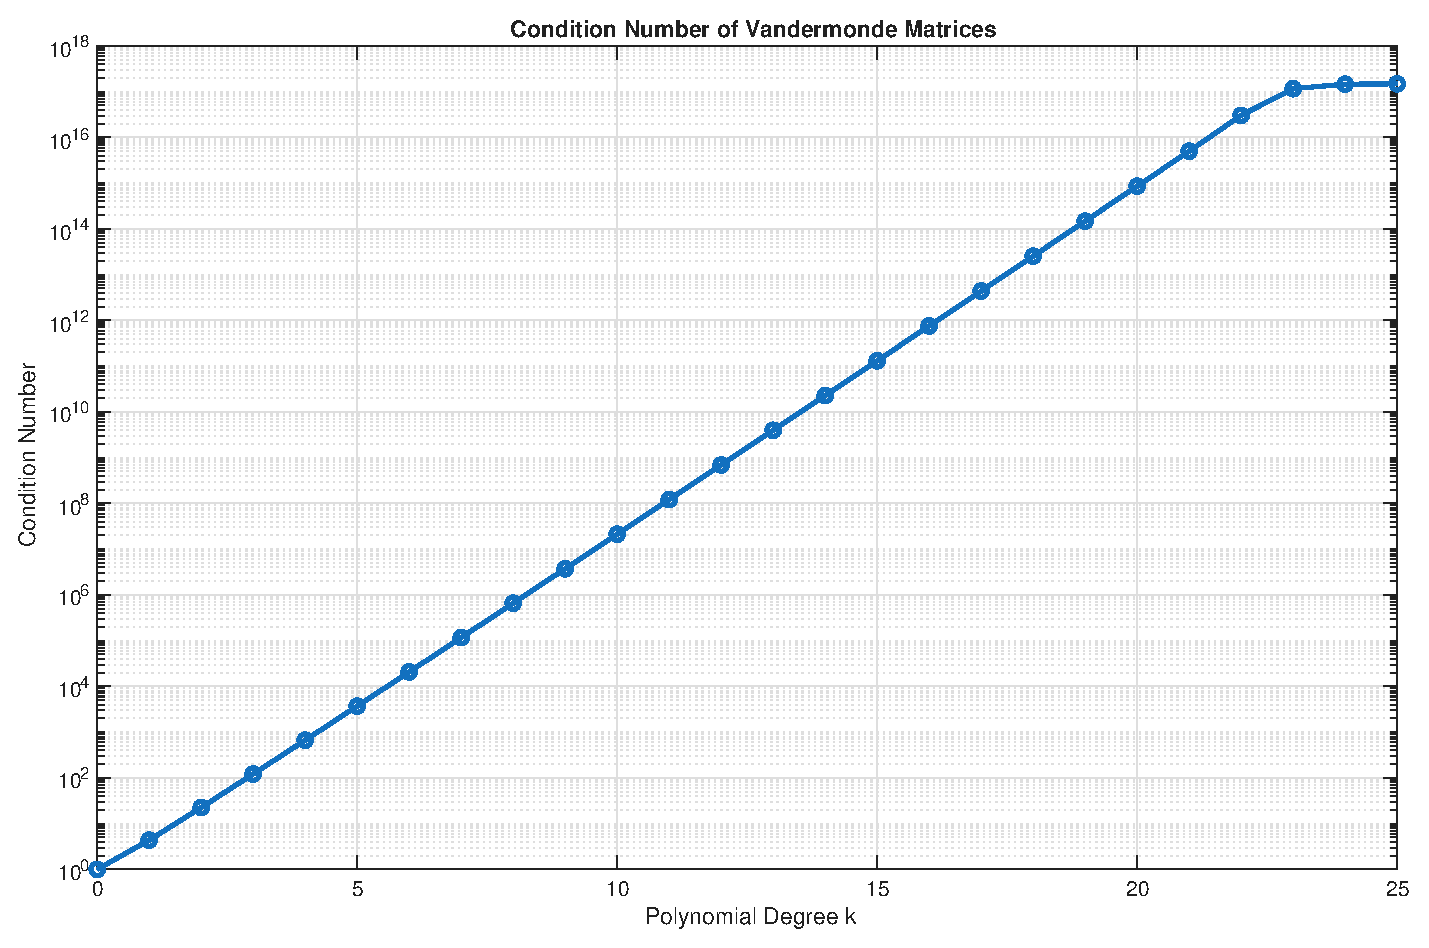
\includegraphics[width=1\textwidth]{Figures/PB_14_1.eps}
    \caption{Condition number of Vandermonde matrices as a function of polynomial degree $k$.}
    \label{fig:vandermonde_cond}
\end{figure}


\subsubsection*{Discussion}
No, it is not better to use more model parameters (a higher degree polynomial) to fit your data. 
As you increase the polynomial degree $k$, the condition number $\kappa(A_k)$ of the Vandermonde matrix grows exponentially. Conditioning is the measure of sensitivity of solutions to perturbations , such as uncertainties or floating-point representation errors in the data. The condition number for finding the least squares solution vector $\vec{x}$ contains the square of the condition number of the matrix $A$, given by the formula $\kappa(A \mapsto \vec{x}) = \kappa(A) + \tan(\theta)\kappa(A)^2\eta$.




%% ============================================================
%% ============================================================
\section*{Appendix: Gemini AI}
\begin{figure}[H]
    \centering
    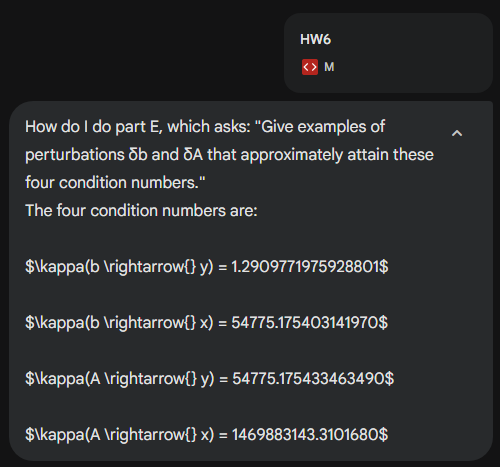
\includegraphics[width=1\linewidth]{image.png}
\end{figure}

\newpage
\section*{Appendix: MATLAB Code}

\lstinputlisting{HW6.m}

\end{document}